Unsupervised learning is a type of machine learning that looks for previously undetected patterns in a data set with no pre-existing labels and with a minimum of human supervision. In contrast to supervised learning that usually makes use of human-labeled data, unsupervised learning, also known as self-organization allows for modeling of probability densities over inputs. It forms one of the three main categories of machine learning, along with supervised and reinforcement learning. Semi-supervised learning, a related variant, makes use of supervised and unsupervised techniques.

\section{K-Means Clustering Algorithm}
	Kmeans algorithm is an iterative algorithm that tries to partition the dataset into K pre-defined distinct non-overlapping subgroups (clusters) where each data point belongs to only one group. It tries to make the intra-cluster data points as similar as possible while also keeping the clusters as different (far) as possible. It assigns data points to a cluster such that the sum of the squared distance between the data points and the cluster’s centroid (arithmetic mean of all the data points that belong to that cluster) is at the minimum. The less variation we have within clusters, the more homogeneous (similar) the data points are within the same cluster.\\\\

	The way kmeans algorithm works is as follows:
	\begin{enumerate}
		\item Specify number of clusters K.
		\item Initialize centroids by first shuffling the dataset and then randomly selecting K data points for the centroids without replacement.
		\item Keep iterating until there is no change to the centroids. i.e assignment of data points to clusters isn’t changing: 
		\begin{itemize}
			\item Compute the sum of the squared distance between data points and all centroids.
			\item Assign each data point to the closest cluster (centroid).
			\item Compute the centroids for the clusters by taking the average of the all data points that belong to each cluster.
		\end{itemize}
	\end{enumerate}

	\subsection{\textbf{The Elbow Method}: Choosing the number of clusters}
		For the k-means clustering method, the most common approach for choosing the number of clusters is the so-called \textbf{elbow method}. It involves running the algorithm multiple times over a loop, with an increasing number of cluster choice and then plotting a clustering score as a function of the number of clusters.\\

		What is the score or metric which is being plotted for the elbow method? Why is it called the ‘elbow’ method?\\

		A typical plot looks like following,

		\begin{figure}[h]
			\centering
			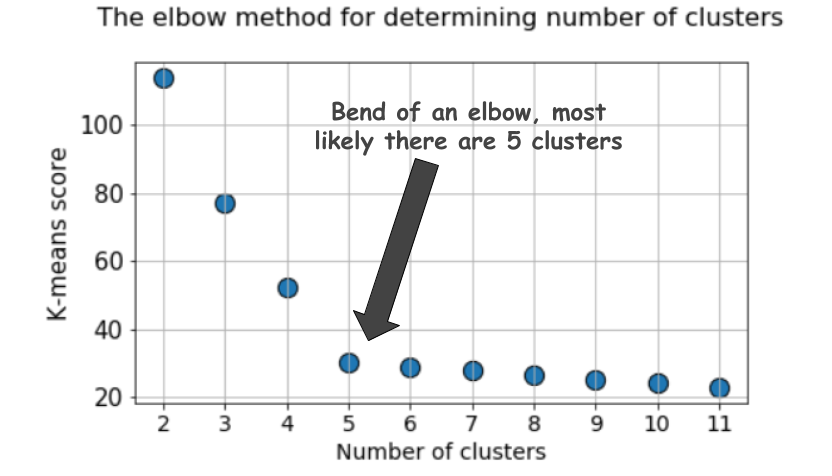
\includegraphics[scale=0.35]{elbow.png}
			\caption{Elbow Method: Score plot}
		\end{figure}

		The score is, in general, a measure of the input data on the k-means objective function i.e. \textbf{some form of intra-cluster distance relative to inner-cluster distance}.

	\subsection{Image compression with K-means}
		In a straightforward 24-bit color representation of an image, each pixel is repre-
		sented as three 8-bit unsigned integers (ranging from 0 to 255) that specify
		the red, green and blue intensity values. This encoding is often refered to as
		the RGB encoding. Our image contains thousands of colors, and in this part
		of the exercise, you will reduce the number of colors to 16 colors.
		By making this reduction, it is possible to represent (compress) the photo
		in an efficient way. Specifically, you only need to store the RGB values of
		the 16 selected colors, and for each pixel in the image you now need to only
		store the index of the color at that location (where only 4 bits are necessary
		to represent 16 possibilities).
		In this exercise, you will use the K-means algorithm to select the 16 colors
		that will be used to represent the compressed image. Concretely, you will
		treat every pixel in the original image as a data example and use the K-means
		algorithm to find the 16 colors that best group (cluster) the pixels in the 3-
		dimensional RGB space. Once you have computed the cluster centroids on
		the image, you will then use the 16 colors to replace the pixels in the original
		image.

		\begin{figure}[h]
			\centering
			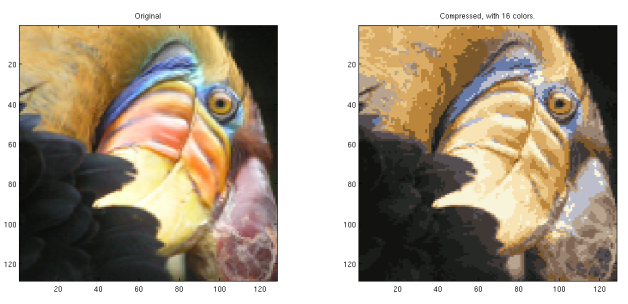
\includegraphics[scale=0.5]{imageCompress.png}
			\caption{Original and Reconstructed Image using K-means}
		\end{figure}		